%%%%%%%%%%%%%%%%%%%%%%%%%%%%%%%%%%%%%%%%%%%%%%%%%%%%%%%%%%%%%%%%%%%%
%% UNSW SENG2020 2012S2 GROUP 6 REPORT TEMPLATE
%% CREATED BY VINCENT WONG
%%%%%%%%%%%%%%%%%%%%%%%%%%%%%%%%%%%%%%%%%%%%%%%%%%%%%%%%%%%%%%%%%%%%

\documentclass[a4paper]{article}
\usepackage[margin=1.5in]{geometry}
%\usepackage{a4wide}
\usepackage{longtable}
\usepackage[normalem]{ulem}     %% gives strikeout capability with \sout{}
\usepackage{graphicx}
\usepackage{float}
\usepackage[usenames,dvipsnames]{color}
\RequirePackage{bsymb,b2latex}
%%%%%%%%%%%%%%%%%%%%%%%%%%%%%%%%%%%%%%%%%%%%%%%%%%%%%%%%%%%%%%%%%%%%%
%% DOCUMENT MACROS -- DO NOT DELETE


\begin{document}

%%%%%%%%%%%%%%%%%%%%%%%%%%%%%%%%%%%%%%%%%%%%%%%%%%%%%%%%%%%%%%%%%%%%%
%% TITLE PAGE
\thispagestyle{empty}      % turn off page numbering
\begin{center}
\Large\textbf{$\odot\int$ Sale} %%\odot \int Sale

\Large\textbf{Design Report}

%%%% MAKE SURE YOU SPECIFY YOUR GROUP NUMBER
\bigskip\large\textbf{Group Number: 06}
\end{center}

\vspace*{16.5cm}
\begin{tabular}{|l|l|}
  \hline
  Version         & 1.0\\\hline
  Print Date      & 15/09/2012 13:37\\\hline
  Release Date    & 15/09/2012\\\hline
  Release State   & Final\\\hline
  Approval State  & Pending\\\hline
  Approved by     & Chris, Dylan, Lasath, Vincent\\\hline
  Prepared by     & Chris, Dylan, Lasath, Vincent\\\hline
  Reviewed by     & Chris, Dylan, Lasath, Vincent\\\hline
  Confidentiality Category  & Public\\\hline
\end{tabular}
\pagebreak

%%%%%%%%%%%%%%%%%%%%%%%%%%%%%%%%%%%%%%%%%%%%%%%%%%%%%%%%%%%%%%%%%%%%%
%% REVISION CONTROL PAGE
\thispagestyle{plain}     % Turn on page numbering
\setcounter{page}{1}      % set page number counter
\renewcommand{\thepage}{\roman{page}}  % set page number to roman

\noindent{\Large\textbf{Document Revision Control}}\\[2ex]
\begin{tabular}{|l|l|l|l|}
  \hline
  Version & Date & Authors & Summary of Changes\\\hline\hline
  0.1 & 03/08/2012     &    Vincent     &    Created initial report               \\\hline
   0.2 & 03/08/2012     &    Lasath     &    Added Architecture section               \\\hline
 
\end{tabular}

\pagebreak

%%%%%%%%%%%%%%%%%%%%%%%%%%%%%%%%%%%%%%%%%%%%%%%%%%%%%%%%%%%%%%%%%%%%%
%% TABLE OF CONTENTS AND FIGURES

\tableofcontents
\pagebreak


%%%%%%%%%%%%%%%%%%%%%%%%%%%%%%%%%%%%%%%%%%%%%%%%%%%%%%%%%%%%%%%%%%%%%
%% MAIN DOCUMENT
\setcounter{page}{1}     % Set page number counter
\renewcommand{\thepage}{\arabic{page}}  % print page number as arabic

%%%%%%%%%%%%%%  THIS IS WHERE YOU PUT YOUR CONTENT %%%%%%%%%%%%%%%%%%

\section{Overview}
The Point of Sale/Warehouse System (PosWare) is designed to be a simple yet sophisticated system that provides extensive sales and logistics management functionality to all kinds of businesses from large to small. 
\\\\
The system will be a distributed system which has various terminals and user interfaces allowing multiple actors in different locations within the store to use the system concurrently. It will also be scalable to suit the needs of different sizes of business, as it can handle the complexity of large chain businesses, while remaining cost effective for small independent stores.
\\\\
The system will incorporate 3 different terminal and user interface designs. This includes the cashier UI, the stock controllers UI and manager UI. They all provide specific layout designed to maximise the efficiency and ease of use for the targeted actor. We have chosen to utilise a prototyping approach in the design of our UI as we constantly release and refine previews of the system based on user feedback. 
\\\\
As the system is designed to suit different businesses, the clients will have an option of choosing their ideal combination of servers and terminals to suite their budgetary needs. They will also be able to opt in for various data redundancy programs such as offsite backups and automatic archiving as they see fit.
\\\\
The majority of the functionality has been modelled using EventB. The backend will stick as close to the model as possible since we understood that the model was constructed to meet the customers requirements, and is internally consistent. The transition is a reasonably straightforward process as outlined in detail later on this document.
\\\\
The following report will outline our final version of our requirements (see appendix) and our complete use case diagram. The report will also provide brief description of the use cases and mapping the various use case to our EventB model in detail. Following this, the report will explain the architecture of our system and the formal specification. Finally our report will provide quick insight into our proposed graphical user interface and the features which our system has to offer.
\pagebreak

\section{Design Considerations}
Our system has to be able to be deployed across multiple machines to suit the needs of medium to large businesses. This allows for cashiers and stock controllers to be in separate locations while working on the same system and also allows multiple cashiers/customers to be active at once (as stated by requirement PD-2.1.1.1). However this does contrast to the capabilities of EventB, which models a single system with a state and purely atomic operations and would be difficult to implement whilst spread over multiple machines.
\\\\
In an attempt to stick as close to the model as possible, we decided to store all state in a database. Since all machines can access this database it essentially allows for a single shared state between the machines.
\\\\
Events were converted into methods (as explained in detail in section 4.0), which will run in a central server. Since all state is maintained within the database, it is unnecessary for these methods/classes to maintain any local state. If fact, doing so is likely to cause unintended consequences or extra side effects. In order to keep these methods atomic, to match model events, they were restricted to one database update query per method (except during rare special circumstances) .
\\\\
Keeping the methods in classes which maintain no state on themselves during execution, whilst allowing us to match the model events, also caused another advantage; they can be executed on different machines. This will allow for good scalability in case of large businesses with lots of machines, they can merely have multiple of servers with distributed load balancing. 
\\\\
This leaves most of the machines as thin clients since they will only need to perform enquiry services rather than individual processing. At this time we are considering making these clients web based for the ease of deployment. 
\\\\
The system will have a backup servers in case issues arise from the system in-store. All the data will be backed up offsite on the users choice of cloud storage provider. The system will be made such that if any issues arise with the onsite servers, requests can be redirected to offsite servers temporarily while the issue gets resolved.The terminals can be replaced if broken as our system has no reliance on the terminal for the system functionality. 
\\\\
We will have 3 key types of user interfaces in this system and each will run on thin clients. These include the Cashiers UI which will be run on the cash registers, Stock controller UI which will be run on back room machines, and the manager UI which can be run anywhere throughout the system. 
\\\\
We also have pay particular attention during the design of the user interface such that it fits into the philosophy we set for this system - simple yet powerful. The user interface should be easy to understand as users will need to be able to use our system without any prior knowledge or reading any sort of user manual. The layout of the system should be clear and straightforward, whilst having messages across the screen guiding users on how to use the system. As stated by requirement PD-4.2.2, the user interface should also have a dedicated help button each screen to aid users in using the system.
\pagebreak

\section{Class Overview }
As explained above, our Stock\_Control\_RX machine was decomposed into several instances of MVC which makes up the core of our system. However for simplicity, they will be referred to as single classes in this section. 
\\\\
Product forms the primary subject of the majority of our requirements and our EventB model. Each instance represents a physical product line sold in store, just as the PRODUCT set from Stock\_Ctx did. A product stores information required to uniquely identify itself as well as cosmetic (non-functional) details to display to the user [PD-1.1.{2,3,4}]. 
However, products need have to have much more data to fulfil most requirements. Thus they are linked to many other objects including suppliers, orders, and sales.
\\\\
As shown in requirements DN-1.1, … , they need to have a stock level associated with them for each stock location. Like the product levels variable in the model, each product instance has an associated stock level with them through stock location. 
\\\\
Each product also has an associated Supplier in order to fulfil requirements PD-1.4.1. Each supplier instance represents an external supplier. They are a subject of Stock Orders, and their primary role is to interact with the system to automatically place a purchase order. Since this step is very hard to model in EventB, it was deemed pointless to model them at all.
\\\\
The rest of our classes are mainly involved with the sales of items and their payments. A dedicated sale class allows us to have many sale items as well as multiple payment transaction for each purchase. The sale class also interact with users which includes both customer and a system user. These combined allow us to meet all the requirements, within our system by directly relating to your EventB.
\\\\
The workers and the customers in the system are represented as users, and all the attributes provide the features that were required by our system. It allowed us to create and edit the users as well as apply discounts for both staff and customers, as described by our requirements for this system.
\pagebreak

\section{Class Diagram}
\begin{figure}[h]
\centering
  \hspace*{-0.3in}
  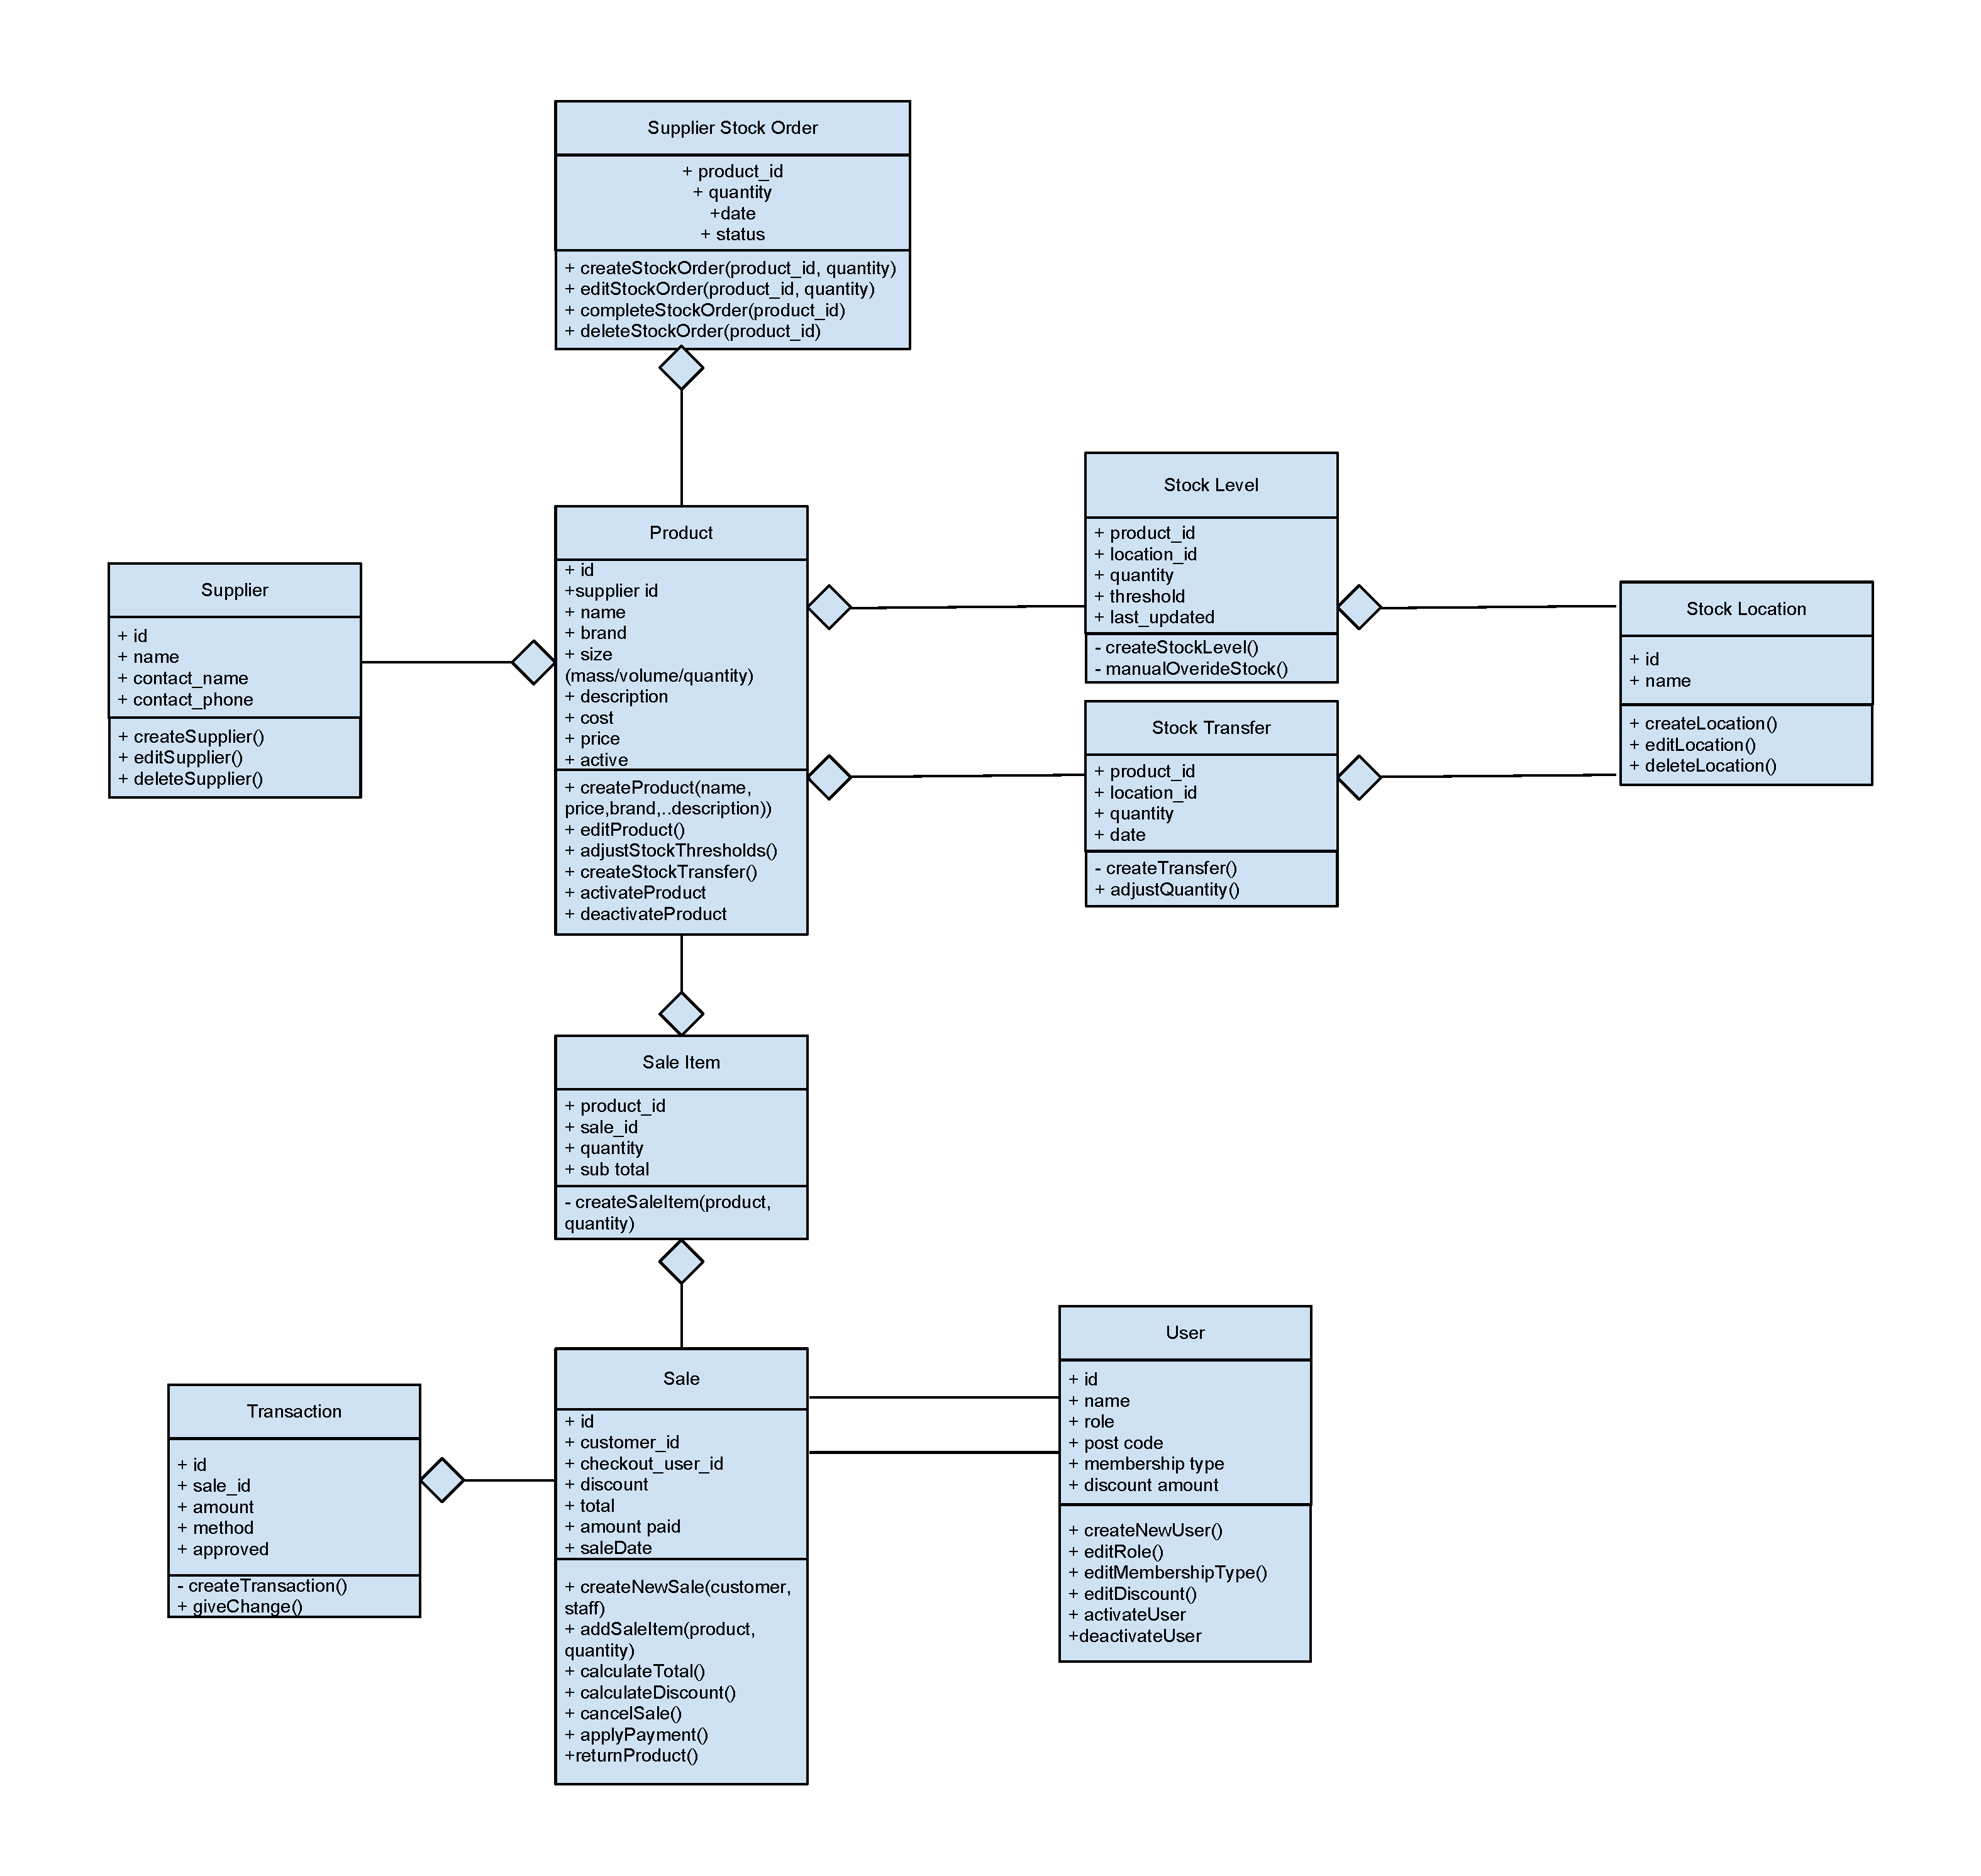
\includegraphics[scale=0.3]{ClassDiagram.pdf}
	\caption{Class diagram designed for superheroes}
\end{figure}

\pagebreak

\section{EventB to Class Mapping}
\pagebreak

\section{EventB Events to Methods}
\pagebreak

\section{System Architecture}

\subsection{Model}

\subsection{View}

\subsection{Controller}

\pagebreak
\section{Sequence Diagrams and Use Cases}

\pagebreak
\section{Design Discussion}

\pagebreak

\section{Appendix}

\appendix

\end{document}

